\subsection{Sơ đồ và đặc tả các trường hợp sử dụng}

\subsubsection{Sơ đồ các trường hợp sử dụng}

Sơ đồ trường hợp sử dụng (use case diagram) cung cấp cái nhìn tổng quan, cấp cao về ranh giới hệ thống và tất cả các chức năng chính mà hệ thống sẽ thực hiện để đáp ứng nhu cầu của các tác nhân. Hình \ref{fig:use-case-diagram} dưới đây minh họa chi tiết mối quan hệ tương tác này trong ngữ cảnh hệ thống của nhóm.

\begin{figure}[H]
    \centering
    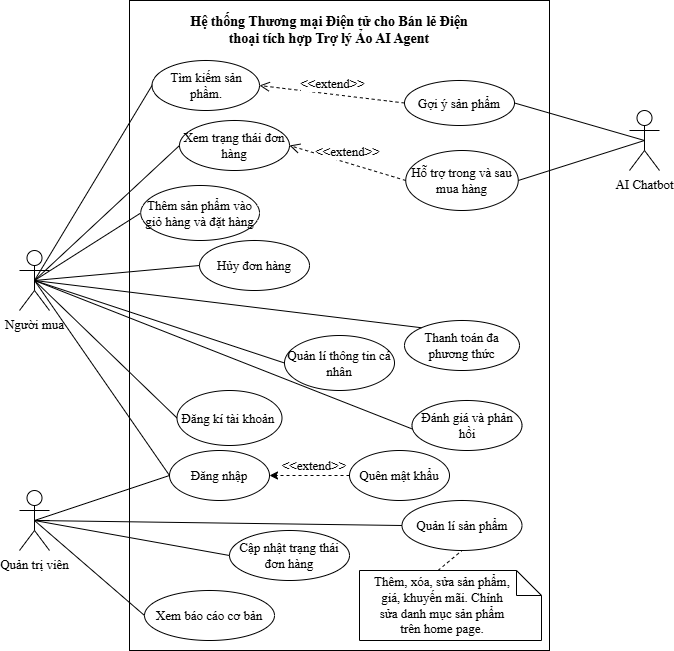
\includegraphics[width=\textwidth]{images/chap3/use_case_diagram/whole_system.png}
    \vspace{0.5cm}
    \caption{Use case diagram tổng thể của hệ thống}
    \label{fig:use-case-diagram}
\end{figure}

\subsubsection{Bảng mô tả chi tiết các trường hợp sử dụng} \label{ss:usecase_detail}

Dựa trên danh mục các yêu cầu chức năng đã xác lập, nhóm tiến hành đặc tả chi tiết các kịch bản tương tác thông qua các bảng mô tả trường hợp sử dụng. Việc đặc tả này nhằm làm rõ trình tự thực hiện, các điều kiện ràng buộc cũng như kết quả mong đợi của từng nghiệp vụ, giúp đảm bảo tính nhất quán giữa khâu phân tích và triển khai thực tế.

Nhằm tối ưu hóa dung lượng của báo cáo và tập trung vào các đặc thù công nghệ của hệ thống, trong phạm vi chương này, nhóm trình bày các mô tả cho những trường hợp sử dụng cốt lõi, bao gồm các nghiệp vụ tìm kiếm sản phẩm, thêm sản phẩm vào giỏ hàng, đặt hàng, thanh toán và các luồng tương tác thông minh với trợ lý ảo AI thông qua các bảng \ref{tab:uc-search-product}, \ref{tab:uc-add-to-cart-checkout}, \ref{tab:uc-multipayment}, \ref{tab:uc-customer-review} và bảng \ref{tab:uc-admin-basic-reports}. Các bảng mô tả chi tiết cho các chức năng quản trị và những nghiệp vụ hỗ trợ khác được trình bày đầy đủ tại phần phụ lục \ref{sec:appx_usecase_detail} của đồ án.

\needspace{3\baselineskip}
\begin{longtable}{|>{\bfseries}p{4cm}|p{11.5cm}|}
\caption{Đặc tả trường hợp sử dụng: Tìm kiếm sản phẩm}
\label{tab:uc-search-product} \\
\hline
\textbf{Tên trường hợp sử dụng} & [UC5] Tìm kiếm sản phẩm \\
\hline
\textbf{Tóm tắt mô tả} & Cho phép khách hàng tìm kiếm sản phẩm theo từ khóa hoặc các tiêu chí bộ lọc. \\
\hline
\textbf{Tác nhân} & Khách hàng. \\
\hline
\textbf{Tiền điều kiện} & 1. Hệ thống hoạt động bình thường. \newline
2. Cơ sở dữ liệu được kết nối với hệ thống. \newline
3. Kết nối với internet được đảm bảo. \\
\hline
\textbf{Sự kiện kích hoạt} & Khách hàng nhập từ khóa vào thanh tìm kiếm hoặc lựa chọn các tiêu chí lọc sản phẩm. \\
\hline
\textbf{Các bước thực hiện} & 1. Khách hàng nhập từ khóa hoặc chọn bộ lọc sản phẩm (giá, cấu hình, hãng...). \newline
2. Hệ thống thực hiện truy vấn cơ sở dữ liệu để tìm kiếm sản phẩm phù hợp. \newline
3. Hệ thống hiển thị danh sách các sản phẩm thỏa mãn điều kiện. \\
\hline
\textbf{Hậu điều kiện} & Danh sách sản phẩm hiển thị phù hợp với tiêu chí tìm kiếm của khách hàng. \\
\hline
\textbf{Luồng thay thế} & Không. \\
\hline
\textbf{Luồng ngoại lệ} & \textbf{Ngoại lệ 1: Tại bước 2} \newline
2a. Nếu xảy ra lỗi kết nối cơ sở dữ liệu, hệ thống thông báo lỗi và yêu cầu người dùng thử lại. \newline
\textbf{Ngoại lệ 2: Tại bước 3} \newline
3a. Nếu không tìm thấy sản phẩm nào phù hợp, hệ thống hiển thị thông báo "Không tìm thấy sản phẩm" kèm theo các gợi ý khác. \\
\hline
\end{longtable}

\needspace{3\baselineskip}
\begin{longtable}{|>{\bfseries}p{4cm}|p{11.5cm}|}
\caption{Đặc tả trường hợp sử dụng: [UC7] Thêm sản phẩm vào giỏ hàng và đặt hàng}
\label{tab:uc-add-to-cart-checkout} \\
\hline
\textbf{Tên trường hợp sử dụng} & Thêm sản phẩm vào giỏ hàng và đặt hàng \\
\hline
\textbf{Tóm tắt mô tả} & Cho phép khách hàng lựa chọn sản phẩm, thêm vào giỏ hàng và thực hiện quy trình đặt hàng với nhiều phương thức thanh toán khác nhau. \\
\hline
\textbf{Tác nhân} & Khách hàng \\
\hline
\textbf{Tiền điều kiện} & 1. Hệ thống hoạt động bình thường. \newline
2. Cơ sở dữ liệu được kết nối với hệ thống. \newline
3. Kết nối với internet được đảm bảo. \newline
4. Sản phẩm còn hàng trong kho. \\
\hline
\textbf{Sự kiện kích hoạt} & Khách hàng chọn sản phẩm và nhấn nút “Thêm vào giỏ hàng” hoặc “Đặt hàng”. \\
\hline
\textbf{Các bước thực hiện} & 1. Khách hàng chọn sản phẩm cần mua. \newline
2. Hệ thống hiển thị chi tiết sản phẩm và nút “Thêm vào giỏ hàng”. \newline
3. Khách hàng thêm sản phẩm vào giỏ. \newline
4. Hệ thống cập nhật giỏ hàng và hiển thị tổng số lượng, giá tiền. \newline
5. Khách hàng chọn “Đặt hàng”. \newline
6. Hệ thống yêu cầu khách hàng xác nhận địa chỉ giao hàng, phương thức thanh toán. \newline
7. Hệ thống kiểm tra tính hợp lệ của thông tin và số lượng tồn kho. \newline
8. Hệ thống tạo đơn hàng và gửi xác nhận cho khách hàng. \\
\hline
\textbf{Hậu điều kiện} & Đơn hàng được tạo thành công và lưu trong hệ thống, khách hàng nhận thông báo xác nhận. \\
\hline
\textbf{Luồng thay thế} & \textbf{Luồng thay thế 1: Tại bước 4} \newline
4a. Khách hàng không đặt hàng ngay mà chỉ thêm sản phẩm vào giỏ hàng và tiếp tục mua sắm. \\
\hline
\textbf{Luồng ngoại lệ} & \textbf{Ngoại lệ 1: Tại bước 6} \newline
6a. Nếu phương thức thanh toán hiện tại không hỗ trợ hoặc xảy ra lỗi cổng thanh toán, hệ thống báo lỗi và yêu cầu khách hàng chọn phương thức thanh toán khác. \\
\hline
\end{longtable}

\needspace{3\baselineskip}
\begin{longtable}{|>{\bfseries}p{4cm}|p{11.5cm}|}
\caption{Đặc tả trường hợp sử dụng: Thanh toán đa phương thức}
\label{tab:uc-multipayment} \\
\hline
\textbf{Tên trường hợp sử dụng} & [UC8] Thanh toán đa phương thức \\
\hline
\textbf{Tóm tắt mô tả} & Cho phép khách hàng thanh toán đơn hàng bằng nhiều phương thức khác nhau như: tiền mặt khi nhận hàng (COD), thẻ ngân hàng, ví điện tử, hoặc các cổng thanh toán trực tuyến. \\
\hline
\textbf{Tác nhân} & Khách hàng. \\
\hline
\textbf{Tiền điều kiện} & 1. Hệ thống hoạt động bình thường. \newline
2. Cơ sở dữ liệu được kết nối với hệ thống. \newline
3. Kết nối với Internet được đảm bảo. \newline
4. Đơn hàng đã được tạo thành công. \newline
5. Hệ thống kết nối thành công với các cổng thanh toán bên thứ ba (nếu có). \\
\hline
\textbf{Sự kiện kích hoạt} & Khách hàng nhấn chọn “Thanh toán” sau khi xác nhận đơn hàng đối với các phương thức trả trước. \\
\hline
\textbf{Các bước thực hiện} & 1. Tùy vào phương thức thanh toán mà khách hàng chọn, hệ thống sẽ hiển thị biểu mẫu hoặc trang thanh toán tương ứng. \newline
2. Khách hàng thực hiện các thao tác thanh toán theo hướng dẫn. \newline
3. Hệ thống hiển thị trạng thái giao dịch và cập nhật trạng thái đơn hàng tương ứng. \\
\hline
\textbf{Hậu điều kiện} & Thanh toán được xử lý thành công và thông tin giao dịch được lưu trữ chính xác trong hệ thống. \\
\hline
\textbf{Luồng thay thế} & \textbf{Luồng thay thế 1: Tại bước 2} \newline
2a. Nếu phương thức thanh toán là “Thanh toán khi nhận hàng” (COD), khách hàng bỏ qua bước thanh toán trực tuyến, hệ thống tự động cập nhật trạng thái đơn hàng sang “Chờ giao hàng”. \\
\hline
\textbf{Luồng ngoại lệ} & \textbf{Ngoại lệ 1: Tại bước 2} \newline
2a. Giao dịch thất bại (sai mã OTP, số dư không đủ...), hệ thống thông báo lỗi và yêu cầu người dùng thử lại hoặc chọn phương thức khác. \newline
2b. Lỗi kết nối với cổng thanh toán bên thứ ba, hệ thống hiển thị thông báo sự cố và giữ đơn hàng ở trạng thái “Chờ thanh toán”. \\
\hline
\end{longtable}

\needspace{3\baselineskip}
\begin{longtable}{|>{\bfseries}p{4cm}|p{11.5cm}|}
\caption{Đặc tả trường hợp sử dụng: Đánh giá và phản hồi của khách hàng}
\label{tab:uc-customer-review} \\
\hline
\textbf{Tên trường hợp sử dụng} & Đánh giá và phản hồi của khách hàng \\
\hline
\textbf{Tóm tắt mô tả} & Khách hàng có thể gửi đánh giá (số sao, nhận xét) về sản phẩm hoặc dịch vụ sau khi nhận hàng để giúp doanh nghiệp cải thiện chất lượng phục vụ. \\
\hline
\textbf{Tác nhân} & Khách hàng. \\
\hline
\textbf{Tiền điều kiện} & 1. Hệ thống hoạt động bình thường. \newline
2. Cơ sở dữ liệu được kết nối với hệ thống. \newline
3. Kết nối với Internet được đảm bảo. \newline
4. Khách hàng đã đăng nhập thành công vào hệ thống. \\
\hline
\textbf{Sự kiện kích hoạt} & Khách hàng nhấn chọn chức năng “Đánh giá” hoặc “Phản hồi” tại danh mục các đơn hàng đã giao thành công. \\
\hline
\textbf{Các bước thực hiện} & 1. Hệ thống hiển thị biểu mẫu đánh giá sản phẩm tương ứng với đơn hàng. \newline
2. Khách hàng thực hiện chọn số sao đánh giá và nhập nội dung nhận xét hoặc góp ý. \newline
3. Hệ thống kiểm tra, thực hiện lưu phản hồi vào cơ sở dữ liệu và gửi thông báo xác nhận thành công. \\
\hline
\textbf{Hậu điều kiện} & Nội dung đánh giá và phản hồi được lưu trữ trong hệ thống và sẵn sàng để hiển thị hoặc phục vụ mục đích báo cáo nội bộ. \\
\hline
\textbf{Luồng thay thế} & \textbf{Luồng thay thế 1: Tại bước 1} \newline
1a. Nếu khách hàng bỏ qua bước đánh giá và thoát màn hình, đơn hàng vẫn được giữ nguyên trạng thái hoàn tất nhưng không có dữ liệu phản hồi kèm theo. \\
\hline
\textbf{Luồng ngoại lệ} & Không. \\
\hline
\end{longtable}

\needspace{3\baselineskip}
\begin{longtable}{|>{\bfseries}p{4cm}|p{11.5cm}|}
\caption{Đặc tả trường hợp sử dụng: Xem báo cáo cơ bản}
\label{tab:uc-admin-basic-reports} \\
\hline
\textbf{Tên trường hợp sử dụng} & Xem báo cáo cơ bản \\
\hline
\textbf{Tóm tắt mô tả} & Cho phép quản trị viên xem báo cáo tổng hợp về doanh thu, số lượng đơn hàng, các sản phẩm bán chạy và phản hồi từ phía khách hàng. \\
\hline
\textbf{Tác nhân} & Quản trị viên. \\
\hline
\textbf{Tiền điều kiện} & 1. Hệ thống hoạt động bình thường. \newline
2. Cơ sở dữ liệu được kết nối với hệ thống. \newline
3. Kết nối với Internet được đảm bảo. \newline
4. Quản trị viên đã đăng nhập thành công vào hệ thống quản trị. \\
\hline
\textbf{Sự kiện kích hoạt} & Quản trị viên nhấn chọn chức năng “Xem báo cáo” hoặc “Thống kê” từ menu điều hướng quản trị. \\
\hline
\textbf{Các bước thực hiện} & 1. Quản trị viên truy cập vào mục quản lý báo cáo và thống kê. \newline
2. Hệ thống hiển thị danh sách các loại báo cáo hiện có (doanh thu theo ngày/tháng, sản phẩm bán chạy, tổng hợp phản hồi khách hàng). \newline
3. Quản trị viên chọn loại báo cáo và các tiêu chí lọc (thời gian, danh mục) cần xem. \newline
4. Hệ thống truy xuất dữ liệu và hiển thị báo cáo dưới dạng bảng số liệu hoặc biểu đồ trực quan. \newline
5. Quản trị viên có thể chọn chức năng xuất báo cáo dưới định dạng PDF hoặc Excel để lưu trữ. \\
\hline
\textbf{Hậu điều kiện} & Quản trị viên nắm bắt được dữ liệu thống kê phục vụ cho việc phân tích kinh doanh và quản lý. \\
\hline
\textbf{Luồng thay thế} & \textbf{Luồng thay thế 1: Tại bước 3} \newline
3a. Quản trị viên thay đổi bộ lọc hoặc tiêu chí thời gian, hệ thống tự động cập nhật lại số liệu báo cáo tương ứng. \\
\hline
\textbf{Luồng ngoại lệ} & \textbf{Ngoại lệ 1: Tại bước 4} \newline
4a. Không có dữ liệu trong khoảng thời gian được chọn, hệ thống hiển thị thông báo “Không có dữ liệu phù hợp”. \newline
4b. Nếu xảy ra lỗi truy xuất dữ liệu từ máy chủ, hệ thống hiển thị thông báo lỗi kỹ thuật. \\
\hline
\end{longtable}

\needspace{3\baselineskip}
\begin{longtable}{|>{\bfseries}p{4cm}|p{11.5cm}|}
\caption{Đặc tả trường hợp sử dụng: Gợi ý sản phẩm}
\label{tab:uc-product-suggestion} \\
\hline
\textbf{Tên trường hợp sử dụng} & Gợi ý sản phẩm \\
\hline
\textbf{Tóm tắt mô tả} & Hệ thống AI ChatBot phân tích hành vi, lịch sử mua sắm và từ khóa tìm kiếm để đưa ra gợi ý sản phẩm cá nhân hóa. Đây là trường hợp sử dụng mở rộng từ “Tìm kiếm sản phẩm”. \\
\hline
\textbf{Tác nhân} & AI ChatBot. \\
\hline
\textbf{Tiền điều kiện} & 1. Hệ thống hoạt động bình thường. \newline
2. Cơ sở dữ liệu được kết nối với hệ thống. \newline
3. Kết nối với internet được đảm bảo. \newline
4. Trường hợp sử dụng “Tìm kiếm sản phẩm” đã được khởi động. \newline
5. Dữ liệu hành vi và lịch sử khách hàng được lưu trữ. \newline
6. AI ChatBot hoạt động và có quyền truy cập dữ liệu sản phẩm. \\
\hline
\textbf{Sự kiện kích hoạt} & Khách hàng tương tác với ChatBot. \\
\hline
\textbf{Các bước thực hiện} & 1. AI ChatBot phân tích từ khóa, lịch sử mua sắm, và hành vi duyệt web của người dùng. \newline
2. Hệ thống hiển thị câu trả lời chứa gợi ý sản phẩm phù hợp ngay trong hộp thoại chat. \\
\hline
\textbf{Hậu điều kiện} & Danh sách gợi ý sản phẩm cá nhân hóa được hiển thị thành công cho khách hàng. \\
\hline
\textbf{Luồng thay thế} & Không. \\
\hline
\textbf{Luồng ngoại lệ} & \textbf{Ngoại lệ 1: Tại bước 1} \newline
1a. Nếu xảy ra lỗi kết nối cơ sở dữ liệu hoặc dịch vụ AI, hệ thống thông báo lỗi và yêu cầu người dùng thử lại. \newline
\textbf{Ngoại lệ 2: Tại bước 2} \newline
2a. Nếu không tìm thấy sản phẩm nào phù hợp với sở thích hoặc lịch sử của người dùng, hệ thống hiển thị thông báo mặc định hoặc gợi ý các sản phẩm phổ biến nhất. \\
\hline
\end{longtable}

\needspace{3\baselineskip}
\begin{longtable}{|>{\bfseries}p{4cm}|p{11.5cm}|}
\caption{Đặc tả trường hợp sử dụng: Hỗ trợ trong và sau mua hàng}
\label{tab:uc-post-purchase-support} \\
\hline
\textbf{Tên trường hợp sử dụng} & Hỗ trợ trong và sau mua hàng \\
\hline
\textbf{Tóm tắt mô tả} & AI ChatBot cung cấp thông tin, tư vấn và giải đáp thắc mắc liên quan đến đơn hàng trong quá trình xử lý hoặc sau khi đã hoàn tất. Đây là trường hợp sử dụng mở rộng từ “Xem trạng thái đơn hàng”. \\
\hline
\textbf{Tác nhân} & AI ChatBot. \\
\hline
\textbf{Tiền điều kiện} & 1. Hệ thống hoạt động bình thường. \newline
2. Cơ sở dữ liệu được kết nối với hệ thống. \newline
3. Kết nối với Internet được đảm bảo. \newline
4. Trường hợp sử dụng “Xem trạng thái đơn hàng” đã được khởi động. \newline
5. AI ChatBot ở trạng thái sẵn sàng phục vụ. \newline
6. Dữ liệu đơn hàng và lịch sử tương tác được lưu trữ đầy đủ trong hệ thống. \\
\hline
\textbf{Sự kiện kích hoạt} & Khách hàng yêu cầu Chatbot hỗ trợ khi đang xem thông tin chi tiết của một đơn hàng. \\
\hline
\textbf{Các bước thực hiện} & 1. Khách hàng nhấn chọn nút “Trợ giúp” hoặc gửi tin nhắn trực tiếp trong giao diện ChatBot. \newline
2. AI ChatBot phân tích nội dung yêu cầu và đưa ra phản hồi tư vấn tự động dựa trên dữ liệu đơn hàng. \\
\hline
\textbf{Hậu điều kiện} & Khách hàng nhận được thông tin hỗ trợ hoặc giải pháp phù hợp cho các vấn đề liên quan đến đơn hàng. \\
\hline
\textbf{Luồng thay thế} & \textbf{Luồng thay thế 1: Tại bước 2} \newline
2a. Nếu khách hàng cần tham khảo các câu hỏi thường gặp (FAQ), AI ChatBot cung cấp liên kết trực tiếp đến trang hướng dẫn hoặc chính sách tương ứng. \\
\hline
\textbf{Luồng ngoại lệ} & \textbf{Ngoại lệ 1: Tại bước 2} \newline
2a. Nếu ChatBot không sẵn dụng hoặc xảy ra lỗi kết nối dịch vụ AI, hệ thống thông báo lỗi và cung cấp phương thức gửi yêu cầu hỗ trợ qua email cho khách hàng. \\
\hline
\end{longtable}
